\documentclass{article}


\usepackage{amsmath, amssymb}
\usepackage{tikz}

\newcommand{\bE}{\mathbb{E}}
\newcommand{\C}{\mathbf{C}}

\title{Notes on the Theory of Multilevel Mediation Analysis with Binary Variables}
\author{William Ruth}
\date{}

\begin{document}

\maketitle

\section{Basic Structure}
\label{sec:basics}

In a mediation model, we have an exposure variable, $X$, a mediator variable, $M$, an outcome variable, $Y$, and a set of confounders, $\mathbf{C}$. In our problem, all variables are categorical. Our assumed causal diagram is given in Figure \ref{fig:causal_diagram}. We see that there is a direct path for $X$ to influence $Y$, as well as an indirect path which is mediated by $M$.

\begin{figure}[t]
    \centering
    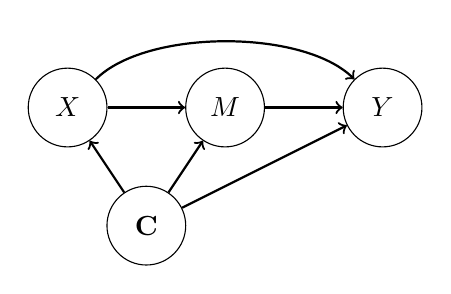
\begin{tikzpicture}
        % Circles
        \node at (0,0) [circle, draw, minimum size=1cm] (X) {$X$};
        \node at (2,0) [circle, draw, minimum size=1cm] (M) {$M$};
        \node at (4,0) [circle, draw, minimum size=1cm] (Y) {$Y$};
        \node at (1, -1.5) [circle, draw, minimum size=1cm] (C) {$\mathbf{C}$};
        
        
        % Arrows
        \draw[->,thick] (X) -- (M);
        \draw[->,thick] (X)  .. controls (1,1) and (3,1) ..  (Y);
        \draw[->,thick] (M) -- (Y);

        \draw[->,thick] (C) -- (X);
        \draw[->,thick] (C) -- (M);
        \draw[->,thick] (C) -- (Y);

    \end{tikzpicture}
    \caption{Causal diagram for our mediation model. See the text for variable definitions.}
    \label{fig:causal_diagram}
\end{figure}%

We model the dependence of $M$ on $X, \mathbf{C}$ and of $Y$ on $X, M, \mathbf{C}$ using logistic regression. Specifically, writing $g$ for the logit link function, we assume that $M$ and $Y$ are Bernoulli distributed with $g(\bE(M | X, \C)) = \alpha_0 + \alpha_1 X + \C \alpha_*$ and $g[\bE(Y | M, X, \C)] = \beta_0 + \beta_1 M + \beta_2 X + \C \beta_*$, where $\alpha_j$ and $\beta_j$ are individual regression coefficients, while $\alpha_*$ and $\beta_*$ are vectors of regression coefficients with length equal to the number of confounders in $\C$. 

The direct, indirect and total effects of $X$ on $Y$ (referred to collectively as the mediation effects) are defined in terms of the above regression coefficients. Respectively, they are $de = \beta_2$, $ie = \alpha_1 \beta_1$ and $te = de + ie = \beta_2 + \alpha_1 \beta_1$. Note that in general it is recommended to also include an interaction term between $M$ and $X$ in the model for $Y$. We did investigate this earlier and found no evidence for a significant effect\footnotemark of this interaction on $\bE Y$, so we thereafter omitted the interaction term from our models.

\footnotetext{We used a likelihood ratio test comparing models with and without the interaction term. The p-value was approximately $0.53$.}

\section{Multi-Level Models}
\label{sec:multi_level}

Our dataset spans 11 different countries. We suspect that the mediation effects may differ across countries. As such, we introduce multilevel structure by adding random effects into our regression models. All variables except the confounders are given country-specific random effects. That is, we re-write our models as $g(\bE(M | X, \C)) = (\alpha_0 + u_0) + (\alpha_1 + u_1) X + \C \alpha_*$ and $g[\bE(Y | M, X, \C)] = (\beta_0 + v_0) + (\beta_1 + v_1) M + (\beta_2 + v_2) X + \C \beta_*$, where $(u_0, u_1) \sim N(0, \Gamma_M)$ and $(v_0, v_1, v_2) \sim N(0, \Gamma_Y)$. Values for these random effects are sampled independently across countries.

Standard mixed-effects regression analysis consists of estimating the $\alpha$s, $\beta$s and $\Gamma$s. However, we are also interested in the values of the country specific random effects. Note that these effects are unobserved random variables, not parameters, so we refer here to prediction of the random effects rather than estimation. Standard approaches for predicting random effects are based on the conditional distribution of these random effects given the observed data (taken one country at a time). That is, for $U = (u_0, u_1)$, we are interested in the law of $U^{(k)} | M^{(k)}$, where the superscript $(k)$ denotes restriction to country $k$. For linear mixed-effects models this conditional law is analytically tractable. However, in the GLMM setting we are forced to operate numerically. Two popular predictors exist: the conditional mean and conditional mode of $U^{(k)}$. The former is theoretically attractive while the latter is more computationally tractable. Existing \texttt{R} software (the \texttt{lme4} package) uses the conditional mode, so that is the approach I have adopted throughout my analysis.

After having obtained predictions for $U$ and $V$ in each country, we can evaluate the corresponding country-specific mediation effects. Note that these mediation effects are defined analogously to those given in Section \ref{sec:basics}, but here the regression coefficients are taken to be mixed effects. The quantities for which we require uncertainty quantification are thus $\hat{de} = \hat{\beta}_2 + \hat{v}_2$, $\hat{ie} = (\hat{\alpha}_1 + \hat{u}_1) (\hat{\beta}_1 + \hat{v}_1)$ and $\hat{te} = \hat{de} + \hat{ie}$.


\section{Bootstrap Uncertainty Quantification}

We use the bootstrap to perform uncertainty quantification for our mediation effects. More specifically, we apply the parametric and non-parametric bootstraps, as well as a new ``semi-parametric'' bootstrap. All three methods involve estimating the sampling distribution of the data, and using this estimate to approximate the sampling distribution of our statistics of interest, $\hat{de}$, $\hat{ie}$ and $\hat{te}$. That is, we approximate the sampling distribution of a statistic, $T$, by first estimating the sampling distribution of the data, then computing the distribution of $T$ under our estimated sampling distribution. Any features of the sampling distribution of $T$ (e.g. standard error) are then estimated from the approximate distribution of $T$. To be precise, we use ``bootstrap distribution'' to refer to the estimated distribution of a sample, and ``bootstrap distribution of $T$'' to refer to the distribution of a statistic, $T$, evaluated on a bootstrap sample\footnotemark. Finally, we can use the bootstrap distribution of $T$ to construct confidence intervals for parameters of the true sampling distribution.

\footnotetext{A few technical notes here. First, formally, the bootstrap distribution is a probability measure on the sample space, while the bootstrap distribution of $T$ is the corresponding pushforward measure induced by $T$ on its range.

Second, note that the bootstrap distribution of a statistic (and of a sample) is a conditional distribution given the observed data. It is therefore a functional statistic. Parameters computed from the bootstrap distribution (e.g. bootstrap mean, variance or confidence intervals) are themselves statistics. One must be careful to distinguish between, e.g., the bootstrap variance of a statistic (i.e. the variance of that statistic's bootstrap distribution) and the sampling variance of that statistic, or, indeed, the sampling variance of the statistic's bootstrap variance.}

In practice, bootstrap distributions are often analytically intractable. Instead, we simulate from the bootstrap distribution and use Monte Carlo techniques to recover quantities of interest. This simulation process typically takes the form of generating a sample from the estimated sampling distribution of the data, then evaluating our statistic on this simulated dataset. Repeating this process a large number of times allows us to closely approximate features of the `true' bootstrap distribution of our statistic. To be completely precise, we use ``bootstrap distribution'' to refer to the distribution of a sample, and ``bootstrap distribution of $T$'' to refer to the distribution of a statistic, $T$, evaluated on

Returning now to our problem, we give three methods for estimating the sampling distribution of the data: parametric, non-parametric and semi-parametric. For each of these methods, we generate a large number of samples from the estimated sampling distribution and compute $\hat{de}$, $\hat{ie}$ and $\hat{te}$ on each of these simulated datasets. This yields a Monte Carlo approximation to the bootstrap distributions of our estimated mediation effects (with a separate approximation for each of the three bootstrap methods). Each of these approximate bootstrap distributions is used to construct a confidence interval for the corresponding true mediation effect in the population. These intervals are constructed using the percentile and basic methods. See below for details.

The rest of this section consists of presenting our three bootstrap methods, then discussing how confidence intervals are constructed from a Monte Carlo bootstrap distribution.



\subsection{Bootstrap Samplers}

In this section, we present the three bootstrap methods used in our analysis: parametric, non-parametric and semi-parametric, and discuss how to simulate datasets under each of these methods.

\subsubsection{Parametric Bootstrap}
\label{sec:par_boot}

The parametric bootstrap begins by estimating model parameters using the observed data. Call these estimates $\hat{\alpha}$, $\hat{\beta}$, $\hat{\Gamma}_M$ and $\hat{\Gamma}_Y$. We then estimate the sampling distribution by plugging-in our estimated parameter values to the parametric family of distributions that we have assumed for the data. That is, we treat the estimated parameters as true parameters, thereby obtaining a particular distribution for the data. This is the parametric bootstrap distribution.

Due to the nested nature of our regression models ($M$ is the response in one model and a covariate in the other), sampling from the parametric bootstrap distribution is a bit intricate. We describe the process here in detail, focusing only on how to simulate data for a single country. Other countries are generated independently using the same method. 

We start by generating random effects for our $M$-model: $U \sim \mathrm{N}(0, \hat{\Gamma}_M)$. For notational simplicity, we pad the vector $U$ with zeros in such a way that $U$ and $\hat{\alpha}$ have the same length, and the terms in $\hat{\alpha}$ without random effects get a zero\footnote{Given the structure of our data and our model, this padding consists of just adding a number of zeros to the end of $U$ equal to the number of confounders.}. Writing $U^+$ for our padded random effects vector, we can express the vector of mixed effects as $\hat{a} = \hat{\alpha} + U^+$. We are now equipped to simulate $M$. To this end, compute the linear predictor, $\eta_M = \hat{a}_0 + \hat{a}_1 X + \C \hat{a}_*$, where $X$ and $\C$ are taken only from the current country. We then compute the corresponding vector of probabilities, $p_M = g^{-1}(\eta_M)$ (recall that $g$ is the logit function), and simulate $M_i \overset{\mathrm{ind}}{\sim} \mathrm{Bernoulli}((p_M)_i)$, with $i$ running from $1$ to the number of people surveyed in the current country.

Upon simulating $M$, we take this vector as a fixed covariate for generating $Y$ and follow the same process. First, simulate random effects $V \sim \mathrm{N}(0, \hat{\Gamma}_Y)$ and pad this vector to match $\hat{\beta}$; call the padded vector $V^+$. Next, compute the vector of mixed effects, $\hat{b} = \hat{\beta} + V^+$, and the linear predictor, $\eta_Y = \hat{b}_0 + \hat{b}_1 M + \hat{b}_2 X + \C \hat{b}_*$. Finally, compute the probabilities, $p_Y = g^{-1}(\eta_Y)$ and simulate $Y_i \overset{\mathrm{ind}}{\sim} \mathrm{Bernoulli}((p_Y)_i)$. We now have a simulated dataset consisting of the fixed covariates, $X$ and $\C$, as well as $M$ and $Y$, for a single country. Repeating this process for all 11 countries gives a single sample from the parametric bootstrap distribution.


\subsubsection{Non-Parametric Bootstrap}

The non-parametric bootstrap is algorithmically much simpler than the parametric one. This method estimates the sampling distribution of the data by the empirical distribution function (EDF). Simulating from the EDF consists of sampling rows from the observed dataset until the size of our `simulated' sample matches the size of our observed dataset. This sampling is performed individually in each country so that the number of people from each country in a bootstrap sample matches the number of people from that country in our original dataset (this equality also holds for the parametric and semi-parametric bootstraps). Sampling in this way from all 11 countries yields a single sample from the non-parametric bootstrap distribution.

\subsubsection{Semi-Parametric Bootstrap}

We observe here that the non-parametric bootstrap involves sampling from the joint distribution of $Y$, $M$, $X$ and $\C$, whereas in the parametric bootstrap sampling is done conditional on $X$ and $\C$. Said differently, every parametric bootstrap sample has identical values of $X$ and $\C$, while in the non-parametric bootstrap the values of these variables are re-arranged in the same way as those of our response variables, $Y$ and $M$.

In order to bridge the gap between these two methods, I propose a ``semi-parametric'' bootstrap. The goal of this method is to incorporate variability in $X$ and $\C$ into the parametric bootstrap without explicitly modelling the sampling distributions of these covariates. The proposed method closely resembles the parametric bootstrap, but adds an additional step at the beginning where $X$ and $\C$ are simulated from their EDFs (i.e. sampled with replacement from the observed data). 

More formally, and focusing only on a single country, the semi-parametric bootstrap estimates the joint distribution of $X$ and $\C$ by their EDF, and the conditional distribution of $Y$ and $M$ given $X$ and $\C$ by our assumed parametric model (i.e. logistic regression). The algorithm begins by deleting $Y$ and $M$ from our dataset and sampling with replacement from the remaining variables, $X$ and $\C$. This gives a sample of the same size as our original dataset for that country, say $\tilde{X}$ and $\tilde{\C}$. We then proceed with the parametric bootstrap sampler for $Y$ and $M$ exactly as described in Section \ref{sec:par_boot}, but with every instance of $X$ and $\C$ replaced by their non-parametrically sampled counterparts, $\tilde{X}$ and $\tilde{\C}$. The parametric bootstrap yields simulated values for $Y$ and $M$ which, when combined with $\tilde{X}$ and $\tilde{\C}$, constitute a semi-parametric bootstrap sample for the country in question. Repeating this process for all 11 countries gives a single sample from the semi-parametric bootstrap sampling distribution.


\subsection{Bootstrap Confidence Intervals}

Regardless of the specific bootstrap method used, we simulate a large number, say $B$, of samples from the bootstrap distribution. On each of these datasets, we estimate the three mediation effects using the method described in Sections \ref{sec:basics} and \ref{sec:multi_level}; write $\hat{de}_b$, $\hat{ie}_b$ and $\hat{te}_b$ for the estimates from bootstrap sample $b$. These calculated mediation effects represent Monte Carlo samples from their respective bootstrap distributions. In this section, we describe two methods for using the Monte Carlo samples to construct confidence intervals for the population-level mediation effects: the percentile and basic methods.

First, the percentile bootstrap confidence interval based on a statistic is constructed using symmetric quantiles from the bootstrap distribution of that statistic. For example, a $95\%$ interval ranges from the $2.5$th to $97.5$th percentiles. In practice, these intervals are constructed using Monte Carlo samples from the bootstrap distribution of the statistic in question. In our problem, we construct $95\%$ confidence intervals for a particular mediation effect, say $de$, by taking the $2.5$th and $97.5$th percentiles of the Monte Carlo sample from the bootstrap distribution of $\hat{de}$.

Note that the percentile confidence interval does not directly use our estimate from the original dataset. The basic interval combines this estimate with percentiles of the bootstrap distribution. Let $m_p$ be the $p$th quantile of the bootstrap distribution for some statistic, and $T$ be the value of that statistic evaluated on the observed data. The basic bootstrap confidence interval is $(2T - m_{0.975}, 2T - m_{0.025})$. 


% \section{Theoretical Justification for Bootstrap Methods}

\end{document}